\documentclass[bibliography=totocnumbered]{scrartcl}

% Codificación
\usepackage[utf8]{inputenc}
\usepackage{natbib}
% Idioma
\usepackage[spanish]{babel}
% Links
\usepackage{hyperref}
\hypersetup{
    colorlinks=true,
    citecolor=black,
    filecolor=black,
    linkcolor=black,
    urlcolor=black
}
% Código de programación
\usepackage{listings}

% SetUp de colores para código
\usepackage{xcolor}

\definecolor{codegreen}{rgb}{0,0.6,0}
\definecolor{codegray}{rgb}{0.5,0.5,0.5}
\definecolor{codepurple}{rgb}{0.58,0,0.82}
\definecolor{backcolour}{rgb}{0.95,0.95,0.92}

\lstdefinestyle{mystyle}{
    %backgroundcolor=\color{backcolour},   
    commentstyle=\color{codegreen},
    keywordstyle=\color{magenta},
    numberstyle=\tiny\color{codegray},
    stringstyle=\color{codepurple},
    basicstyle=\ttfamily\footnotesize,
    breakatwhitespace=false,         
    breaklines=true,                 
    captionpos=b,                    
    keepspaces=true,                 
    %numbers=left,                    
    numbersep=5pt,                  
    showspaces=false,                
    showstringspaces=false,
    showtabs=false,                  
    tabsize=2
}
\lstset{style=mystyle}

% Cambios de color para links
\newcommand{\changeurlcolor}[1]{\hypersetup{urlcolor=#1}}       

% Imágenes
\usepackage{graphicx}

\title{SQL injection}
%\subtitle{subtitle}
\author{Víctor Nieves Sánchez}
\date{Última modificación \today{}}

\begin{document}
\maketitle
\section*{Disclaimer}
Este documento se ha elaborado por los autores, obteniendo información de diversos recursos, principalmente de la página web de \changeurlcolor{blue}\href{https://portswigger.net/web-security}{\textit{PortSwigger}}.\\

El objetivo de este documento es proporcionar una breve referencia de ayuda para el lector.\\

Si deseas más información, os recomendamos realizar los labs de su página web:
\begin{center}
\changeurlcolor{blue}\href{https://portswigger.net/web-security}{https://portswigger.net/web-security}    
\end{center}

\newpage
\tableofcontents

\newpage
\listoffigures

\newpage

\section{¿Qué es SQL injection?}
Normalmente conocida como \textit{SQLi} es una vulnerabilidad que permite al atacante interferir en las consultas que la aplicación hace a la base de datos. Generalmente permite al atacante obtener información la cual normalmente un usuario no tiene acceso. Esto puede incluir información de otro usuario o cualquier información de la aplicación que esté almacenada en la base de datos. En muchos casos, el atacante puede modificar o eliminar los registros que existen en la base de datos.\\

En algunas situaciones, la vulnerabilidad se puede escalar hasta comprometer el propio servidor o realizar un ataque \textit{Denial-of-Service (DoS)}.

\begin{figure}[h]
  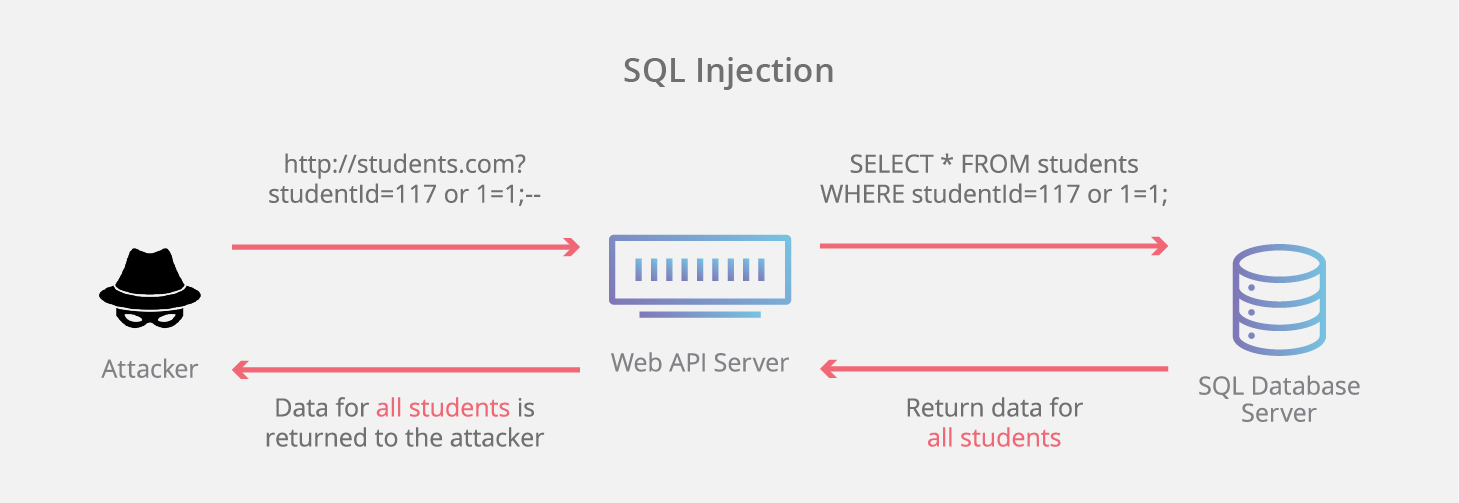
\includegraphics[width=\linewidth]{figures/SQLi.png}
  \caption{Esquema de SQLi}
  \label{fig:SQLi1}
\end{figure}

\section{Ejemplos de SQLi}
Hay una gran variedad de SQLi, ataques y técnicas, dependiendo de la situación concreta. Algunos de los ejemplos más comunes se explicarán a continuación.

\subsection{Obtención de datos ocultos}
Considera una aplicación de compras que muestra productos de diferentes categorías. Cuando el usuario clica en una categoría concreta \textit{C1}, la petición URL será parecida a:
\begin{center}
\nolinkurl{https://website.com/productos?categoria=C1}
\end{center}
Esta petición genera una consulta SQL que devuelve la lista de productos de la categoría concreta. La consulta puede ser algo parecido a:
\begin{lstlisting}[language=SQL]
        SELECT * FROM productos WHERE categoria = 'C1' AND stock = 1
\end{lstlisting}
Esta consulta pide a la base de datos que devuelva todos los detalles \textit{(*)} de la tabla \textit{productos} cuya categoría sea \textit{C1} y estén en \textit{stock}.\\
La restricción \textit{stock = 1} se está usando para mostrar solo los elementos que están en stock, ocultando los que no estén (\textit{stock = 0}).\\

Considerando que la aplicación no implementa ninguna defensa frente SQLi, podemos construir un ataque como
\begin{center}
\nolinkurl{https://website.com/productos?categoria=C1'--}
\end{center}
Por lo que la consulta a la base de datos resultante sería:
\begin{lstlisting}[language=SQL]
        SELECT * FROM productos WHERE categoria = 'C1'--' AND stock = 1
\end{lstlisting}
La calve está en que el elemento \textit{\texttt{--}} es un indicador de comentario en SQL, y esto implica que lo que está a la derecha de éste simbolo se interprete como un comentario, por lo que la restricción deja de formar parte de la consulta.\\

Avanzando un poquito más, podemos conseguir que la aplicación nos devuelva todos los productos de todas las categorías. Para ello, construimos una consulta de la siguiente manera
\begin{center}
\nolinkurl{https://website.com/productos?categoria=C1'+OR+1=1--}
\end{center}
La consulta resultante sería:
\begin{lstlisting}[language=SQL]
  SELECT * FROM productos WHERE categoria = 'C1' OR 1=1--' AND stock = 1
\end{lstlisting}
Por lo que la respuesta nos devolverá todos los elementos que sean de la categoría \textit{C1} o que cumplan la condición \textit{1=1}, y como esta condición es siempre cierta, nos devolverá todos los productos.\\

\subsection{Modificar la lógica de la aplicación}
Consideremos una aplicación que permite a los usuarios iniciar sesión con su usuario y su contraseña, y que la consulta SQL tiene la siguiente forma:
\begin{lstlisting}[language=SQL]
 SELECT * FROM usuarios WHERE username='username' AND password='password'
\end{lstlisting}
Si la consulta retorna los datos del usuario, entonces éste ha iniciado sesión correctamente, pero si los datos no son correctos, se rechazará el inicio de sesión.\\

Un atacante puede iniciar sesión usando los caracteres de comentario en SQL \textit{(\texttt{--})} para eliminar la condición de la contraseña. Por ejemplo, supongamos que existe un usuario con \textit{username} "\textit{administrator}". Se podría construir un ataque que nos permita iniciar sesión con este usuario sin necesidad de saber la contraseña.
\begin{lstlisting}[language=SQL]
 SELECT * FROM usuarios WHERE username='administrator'--' AND password=''
\end{lstlisting}

\subsection{Obtención de información de otras tablas}



\newpage
NO SON REFERENCIAS REALES, SON DE EJEMPLO
% Citar todas las ref (incluidas las que no han sido citadas)
\nocite{*}
\bibliographystyle{plain}
\bibliography{referencias}

\end{document}

